\documentclass[11pt,a4paper,fontset=none]{ctexart}
\usepackage[margin=2.2cm]{geometry}
\usepackage{fontspec}
\newcommand{\WinFonts}{/mnt/c/Windows/Fonts/}
\IfFontExistsTF{Times New Roman}{\setmainfont{Times New Roman}\setsansfont{Times New Roman}}{%
  \IfFileExists{\WinFonts times.ttf}{\setmainfont{times.ttf}[Path=\WinFonts, BoldFont=timesbd.ttf, ItalicFont=timesi.ttf]%
    \setsansfont{times.ttf}[Path=\WinFonts, BoldFont=timesbd.ttf]}{\setmainfont{TeX Gyre Termes}\setsansfont{TeX Gyre Termes}}}
\newcommand{\KaiPath}{/System/Library/AssetsV2/com_apple_MobileAsset_Font8/88d6cc32a907955efa1d014207889413890573be.asset/AssetData/}
\IfFileExists{\KaiPath Kaiti.ttc}{%
  \setCJKmainfont{Kaiti.ttc}[Path=\KaiPath, FontIndex=0, BoldFont=Kaiti.ttc, BoldFeatures={FontIndex=3}]
  \setCJKsansfont{Kaiti.ttc}[Path=\KaiPath, FontIndex=0, BoldFont=Kaiti.ttc, BoldFeatures={FontIndex=3}]
  \setCJKmonofont{Kaiti.ttc}[Path=\KaiPath, FontIndex=0]}{%
  \IfFontExistsTF{Kaiti SC}{\setCJKmainfont{Kaiti SC}\setCJKsansfont{Kaiti SC}\setCJKmonofont{Kaiti SC}}{%
  \IfFileExists{\WinFonts simkai.ttf}{\setCJKmainfont{simkai.ttf}[Path=\WinFonts, AutoFakeBold=2.5]\setCJKsansfont{simkai.ttf}[Path=\WinFonts, AutoFakeBold=2.5]%
    \setCJKmonofont{simkai.ttf}[Path=\WinFonts]}{%
  \setCJKmainfont{FandolKai-Regular.otf}[AutoFakeBold=2.5]\setCJKsansfont{FandolKai-Regular.otf}[AutoFakeBold=2.5]%
  \setCJKmonofont{FandolKai-Regular.otf}}}}% by file name: TeX Live's own fonts are not known to fontconfig on Linux
\usepackage{amsmath}
\usepackage{booktabs,tabularx,longtable,array,graphicx,float}
\usepackage{enumitem}
\usepackage{xurl}
\usepackage[hidelinks]{hyperref}
\usepackage{fancyhdr}
\setlist{nosep,leftmargin=1.4em}
\ctexset{section={format=\Large\bfseries\raggedright},subsection={format=\large\bfseries\raggedright}}
\setlength{\parskip}{0.3em}
\renewcommand{\arraystretch}{1.15}
\pagestyle{fancy}\fancyhf{}
\lhead{\small BAI AI Lab mmBench 多模态评测}\rhead{\small 2026-10-31}\cfoot{\small\thepage}
\renewcommand{\headrulewidth}{0.4pt}

\begin{document}
\begin{center}
{\LARGE\bfseries mmBench 多模态评测报告}\\[0.5em]
{\Large MiniMax M3.1 Flash / DeepSeek Flash V4.1-1017 / Kimi K3.1 Pro}\\[0.4em]
{\small 2026-10-31}
\end{center}
\section{总结}
在 354 道题（7 项能力：学科推理、视觉感知、图表、文档、空间、界面定位、视频时序）上，按各项等权的总分：第 1 名 Kimi K3.1 Pro 85.3（81.9–88.6）；第 2 名 MiniMax M3.1 Flash 74.5（70.6–78.2）；第 2 名 DeepSeek Flash V4.1-1017 73.7（70.1–77.5）（括号内为 95\% 区间）。Kimi K3.1 Pro 比 MiniMax M3.1 Flash 高 10.9 分（区间 +8.0 至 +13.7），差距显著；逐题比较 90 题更好、15 题更差、249 题相同（符号检验 p < 0.001）。MiniMax M3.1 Flash 比 DeepSeek Flash V4.1-1017 高 0.7 分（区间 -1.9 至 +3.5），区间包含 0，判为平手；逐题比较 55 题更好、52 题更差、247 题相同（符号检验 p = 0.847）。Kimi K3.1 Pro 最强的是空间（93.5），最弱的是图表（76.0）。MiniMax M3.1 Flash 最强的是视频时序（85.5），最弱的是界面定位（57.5）。DeepSeek Flash V4.1-1017 最强的是文档（87.1），最弱的是界面定位（36.5）。
\par 说明：
\begin{itemize}
\item 每道题每个模型答 4 次，题目得分取各次的平均；只比较所有模型都答过的 354 道题。题目抽自公开评测集，按来源的难度分为 L1–L4，分数不能和这些评测集的官方榜单直接比较。
\item 总分是各项能力的等权平均，不按题数加权。95\% 区间来自 2000 次按题重抽样（bootstrap）；两两差值的区间在每项能力内成对重抽样。区间包含 0 的两个模型判为平手，名次相同。
\item 按这套题的题量，两两总分差的 95\% 区间半宽约 ±2.7 分：比这小的差距分不出来。
\item MiniMax M3.1 Flash：max\_tokens 不设上限，temperature 用厂商默认值。
\item DeepSeek Flash V4.1-1017：reasoning\_effort = max，max\_tokens = 96000，temperature 用厂商默认值。
\item Kimi K3.1 Pro：reasoning\_effort = max，max\_tokens = 96000，temperature 用厂商默认值。
\end{itemize}
\section{模型简介}
各模型的发布信息、相较上一版的更新与亮点，整理自厂商公告与模型卡；标注“厂商自报”的分数未经独立复现，与本报告的测评结果不是同一口径。
\subsection*{MiniMax M3.1 Flash}
\begin{center}\small
\resizebox{\ifdim\width>\linewidth\linewidth\else\width\fi}{!}{%
\begin{tabular}{@{}p{2.2cm}>{\raggedright\arraybackslash}p{13.6cm}@{}}
\toprule
项目 & 内容 \\
\midrule
厂商 & MiniMax \\
发布 & 2026-09-27 以 M3.1-Flash-Preview 在 MiniMax Code 内测；2026-10-19 正式上线 API；2026-10-23 放出权重 \\
权重与许可 & 开放权重，MiniMax Community License（商用须标注；年收入 2000 万美元以上须书面授权） \\
架构 & MoE：总参数约 428B、每 token 激活约 23B（与 M3 同规模），官方称采用更激进的稀疏化；上下文 1M；输入文本、图像、视频；思考不能关闭，深度用 reasoning\_effort 调（默认 max） \\
价格 & 每百万 token 输入 \$0.15、缓存 \$0.015、输出 \$0.60，不分时段、不分上下文长度（国内站 ¥1 / ¥0.1 / ¥4） \\
本次调用 & MiniMax 官方 API（国内站，OpenAI 兼容接口） \\
\bottomrule
\end{tabular}}
\end{center}
相较上一版的更新：
\begin{itemize}
\item 官方称在线推理速度快了近 3 倍，智能体任务的整体使用成本比前代低 70\%（博客未点名前代）；输出速度可达 200+ token/s，P50 在 170+
\item 2026-10-19 起 MiniMax 把 M2.5、M2.7 归为旧版，套餐内对它们的请求自动改由 M3.1 Flash 处理
\end{itemize}
亮点：
\begin{itemize}
\item 定位智能体任务：长程软件工程、电脑操作、企业流程自动化、网络安全
\item 厂商自报 DeepSWE v1.1 73.7\%、OSWorld V2 61.7、Agents' Last Exam 29.6、CyberGym 82\%
\item 单价是同档最低的一批；第三方测评提示其幻觉率偏高，答案需要核验
\end{itemize}
{\small 资料来源：\href{https://www.minimax.io/blog/minimax-m31f}{MiniMax 官方博客：M3.1 Flash}；\href{https://platform.minimax.io/docs/guides/text-generation}{MiniMax 接口文档}；\href{https://www.orcarouter.ai/blog/minimax-m3-1-flash-open-weights}{权重与许可（OrcaRouter 汇总）}；\href{https://venturebeat.com/technology/minimaxs-new-m3-1-flash-beats-deepseek-and-opus-5-on-a-key-business-benchmark-at-lower-cost-but-with-a-high-hallucination-rate}{VentureBeat：幻觉率}}
\subsection*{DeepSeek Flash V4.1-1017}
\begin{center}\small
\resizebox{\ifdim\width>\linewidth\linewidth\else\width\fi}{!}{%
\begin{tabular}{@{}p{2.2cm}>{\raggedright\arraybackslash}p{13.6cm}@{}}
\toprule
项目 & 内容 \\
\midrule
厂商 & DeepSeek \\
发布 & V4.1-Flash 2026-09-10 发布；2026-10-17 更新为 1017 版（API 名 deepseek-flash 与价格不变） \\
权重与许可 & 开放权重，MIT 许可 \\
架构 & 多模态 MoE：主干 552B 参数，每 token 激活 8B（prefill）/ 16B（decode），另有 196B Engram 条件记忆；上下文 1M；支持图像输入 \\
价格 & 每百万 token 输入 \$0.30、缓存命中 \$0.006、输出 \$1.20；北京时间非高峰时段半价 \\
本次调用 & DeepSeek 官方 API \\
\bottomrule
\end{tabular}}
\end{center}
相较上一版的更新：
\begin{itemize}
\item 1017 版相较 9 月版：官方称缩短了任务耗时和输出长度；厂商自报 Terminal-Bench 4.0 31.2 → 42.3、DeepSWE v1.1 74.2 → 77.0、ProgramBench 20.3 → 29.1、NL2Repo-Bench 65.4 → 68.2、HLE（无工具）36.8 → 42.6
\item V4.1 代相较 V4-Flash：新架构系列里最小的模型，原生支持视觉理解；持久 KV cache 约为 V4-Flash 的 1/8，全局 KV cache 每 token 890 字节、约为 1/4；Codeforces 评分 3289 → 3471（厂商自报，各次测评环境不完全相同）
\end{itemize}
亮点：
\begin{itemize}
\item 开放权重、MIT 许可，单价在同档里偏低，非高峰再打对折
\item 1M 上下文，思考深度可调（API 提供 low / high / max）
\item 厂商自报 DeepSWE v1.1 77.0、Terminal-Bench 4.0 42.3，偏重智能体编程
\end{itemize}
{\small 资料来源：\href{https://api-docs.deepseek.com/updates/}{DeepSeek API 更新日志}；\href{https://huggingface.co/deepseek-ai/DeepSeek-V4.1-Flash}{DeepSeek-V4.1-Flash 模型卡}}
\section{能力画像}
每项能力的得分是该项各题得分的平均（0–100）。
\begin{figure}[H]\centering
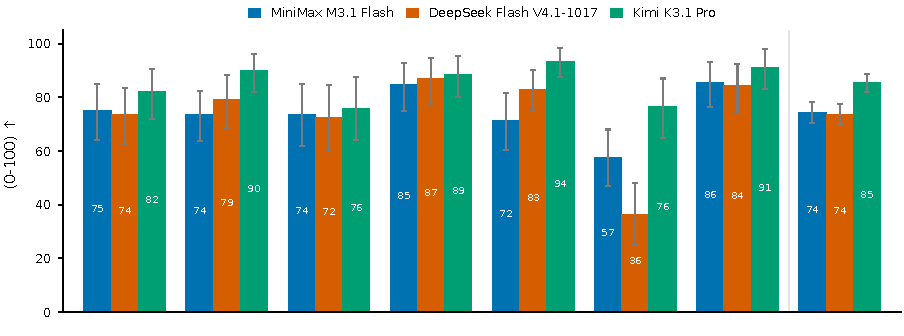
\includegraphics[width=1\linewidth]{fig_profile.pdf}
\caption{各项能力得分（误差线为 95\% 区间）}
\end{figure}
\begin{center}\small
\resizebox{\ifdim\width>\linewidth\linewidth\else\width\fi}{!}{%
\begin{tabular}{lrrrr}
\toprule
 &  & \multicolumn{3}{c}{得分（0–100，括号内 95\% 区间）↑} \\ \cmidrule(lr){3-5}
能力 & 题数 & MiniMax M3.1 Flash & DeepSeek Flash V4.1-1017 & Kimi K3.1 Pro \\
\midrule
学科推理 & 50 & 75.0（64.0–85.0） & 73.5（62.5–83.5） & 82.0（72.0–90.5） \\
视觉感知 & 54 & 73.6（63.9–82.4） & 79.2（68.5–88.4） & 89.8（81.9–96.3） \\
图表 & 50 & 73.5（62.0–85.0） & 72.5（60.5–84.5） & 76.0（64.0–87.5） \\
文档 & 50 & 84.8（75.0–92.7） & 87.1（77.5–94.6） & 88.6（80.1–95.4） \\
空间 & 50 & 71.5（60.5–81.5） & 83.0（75.0–90.0） & 93.5（87.5–98.5） \\
界面定位 & 50 & 57.5（47.0–68.0） & 36.5（25.0–48.0） & 76.5（65.0–87.0） \\
视频时序 & 50 & 85.5（76.5–93.0） & 84.5（74.5–92.5） & 91.0（83.0–98.0） \\
总分（等权） & 354 & 74.5（70.6–78.2） & 73.7（70.1–77.5） & 85.3（81.9–88.6） \\
\bottomrule
\end{tabular}}
\end{center}
\section{排名}
名次 = 1 + 明显强于它的模型数；区间包含 0 的模型名次相同。
\begin{center}\small
\resizebox{\ifdim\width>\linewidth\linewidth\else\width\fi}{!}{%
\begin{tabular}{llr}
\toprule
名次 & 模型 & 总分 ↑ \\
\midrule
1 & Kimi K3.1 Pro & 85.3（81.9–88.6） \\
2 & MiniMax M3.1 Flash & 74.5（70.6–78.2） \\
2 & DeepSeek Flash V4.1-1017 & 73.7（70.1–77.5） \\
\bottomrule
\end{tabular}}
\end{center}
两两比较：总分差与 95\% 区间；逐题比较的胜、负、平题数与符号检验。
\begin{center}\small
\resizebox{\ifdim\width>\linewidth\linewidth\else\width\fi}{!}{%
\begin{tabular}{lrrrrrr}
\toprule
比较 & 总分差 & 95\% 区间 & 胜 & 负 & 平 & p \\
\midrule
Kimi K3.1 Pro − MiniMax M3.1 Flash & +10.9 & +8.0 至 +13.7 & 90 & 15 & 249 & < 0.001 \\
Kimi K3.1 Pro − DeepSeek Flash V4.1-1017 & +11.6 & +9.0 至 +14.5 & 79 & 8 & 267 & < 0.001 \\
MiniMax M3.1 Flash − DeepSeek Flash V4.1-1017 & +0.7 & -1.9 至 +3.5 & 55 & 52 & 247 & 0.847 \\
\bottomrule
\end{tabular}}
\end{center}
\section{按难度}
各档的题来自不同评测集（见下表），这里把所有能力合在一起按题平均。
\begin{center}\small
\resizebox{\ifdim\width>\linewidth\linewidth\else\width\fi}{!}{%
\begin{tabular}{lrrrr}
\toprule
 &  & \multicolumn{3}{c}{得分 ↑} \\ \cmidrule(lr){3-5}
难度 & 题数 & MiniMax M3.1 Flash & DeepSeek Flash V4.1-1017 & Kimi K3.1 Pro \\
\midrule
L1 基础 & 96 & 90.0 & 88.1 & 92.8 \\
L2 中等 & 107 & 73.6 & 78.7 & 87.1 \\
L3 困难 & 151 & 65.2 & 61.3 & 79.5 \\
\bottomrule
\end{tabular}}
\end{center}
\section{按来源}
每个来源评测集上的得分，只是抽样的子集，不等于该评测集的完整成绩。
\begin{center}\small
\resizebox{\ifdim\width>\linewidth\linewidth\else\width\fi}{!}{%
\begin{tabular}{lllrrrr}
\toprule
 &  &  &  & \multicolumn{3}{c}{得分 ↑} \\ \cmidrule(lr){5-7}
能力 & 来源 & 难度 & 题数 & MiniMax M3.1 Flash & DeepSeek Flash V4.1-1017 & Kimi K3.1 Pro \\
\midrule
学科推理 & mmmu\_pro & L1/L2/L3 & 50 & 75.0 & 73.5 & 82.0 \\
视觉感知 & blink & L2 & 54 & 73.6 & 79.2 & 89.8 \\
图表 & chartqa & L1 & 15 & 86.7 & 86.7 & 86.7 \\
图表 & charxiv & L3 & 35 & 67.9 & 66.4 & 71.4 \\
文档 & docvqa & L1 & 30 & 93.8 & 94.3 & 94.4 \\
文档 & ocrbench\_kie & L2 & 20 & 71.3 & 76.2 & 79.9 \\
空间 & blink\_spatial & L2 & 16 & 71.9 & 79.7 & 87.5 \\
空间 & cvbench\_3d & L1 & 14 & 92.9 & 98.2 & 98.2 \\
空间 & mindcube & L3 & 20 & 56.2 & 75.0 & 95.0 \\
界面定位 & screenspot\_pro & L3 & 30 & 35.0 & 8.3 & 60.8 \\
界面定位 & screenspot\_v2 & L1 & 20 & 91.2 & 78.8 & 100.0 \\
视频时序 & timeblind & L3 & 50 & 85.5 & 84.5 & 91.0 \\
\bottomrule
\end{tabular}}
\end{center}
\section{成本与速度}
\begin{center}\small
\resizebox{\ifdim\width>\linewidth\linewidth\else\width\fi}{!}{%
\begin{tabular}{lrrrrrr}
\toprule
模型 & 调用次数 & 平均输入 token ↓ & 平均输出 token ↓ & 延迟中位数 s ↓ & 总费用 ↓ & 每题费用 ↓ \\
\midrule
MiniMax M3.1 Flash & 1416 & 5.4k & 1.8k & 4 & \$2.17 & \$0.006 \\
DeepSeek Flash V4.1-1017 & 1416 & 2.3k & 4.7k & 6 & \$8.25 & \$0.023 \\
Kimi K3.1 Pro & 1416 & 6.0k & 0.9k & 11 & – & – \\
\bottomrule
\end{tabular}}
\end{center}
\section{评分规则}
\begin{center}\small
\resizebox{\ifdim\width>\linewidth\linewidth\else\width\fi}{!}{%
\begin{tabular}{@{}p{2.2cm}>{\raggedright\arraybackslash}p{13.6cm}@{}}
\toprule
题型 & 怎么判 \\
\midrule
选择题 & 取回答最后一行 “Answer: X” 中的选项字母，与标准答案相同得 1 分 \\
是 / 否 & 取最后的 yes 或 no，与标准答案相同得 1 分 \\
短答案 & 标准答案是数字时，取回答里的数（可以带单位或 million、billion 等量级词，按量级换算或不换算都算），相对误差 1\% 内（ChartQA 按其规则放宽到 5\%）得 1 分；文字答案规范化（小写、去冠词和标点）后完全相同得 1 分 \\
文档问答 & ANLS：与最接近的标准答案的归一化编辑距离相似度，低于 0.5 记 0（DocVQA 的规则） \\
界面定位 & 模型给出 0–1000 的相对坐标，换算到原图后落在目标框内得 1 分 \\
视频 & 所有模型都拿到同样的若干帧（按时间均匀抽取的图片），按上面的题型判分 \\
\bottomrule
\end{tabular}}
\end{center}
\par\vspace{2em}\begin{flushright}由 Albert Huang 创建于 2026-10-31\end{flushright}
\end{document}
